% chapter17.tex -- Conclusion
% Based on the author's UGThesis.docx.

\chapter{Conclusion}
\label{ch:conclusion}

In this thesis we have presented the first algorithm for generating all triangulations of a biconnected plane graph in \(O(1)\) amortised time per triangulation and \(O(n)\) space. 
Our algorithm extends the elegant genealogical tree framework of Parvez, Rahman, and Nakano~\cite{parvez2011} from triconnected to biconnected graphs by introducing three key innovations: safe root vertex selection, local genealogical trees with dynamic global chord management, and a pruning strategy based on the persistence of non-root chords.

\section{Summary of Contributions}
\label{sec:contributions}

We now summarise the main contributions of this thesis.

\begin{enumerate}
    \item \textbf{Extension to biconnected graphs:} 
    We overcame the multi-edge problem caused by separation pairs, which had prevented the direct application of the triconnected algorithm. 
    By processing faces sequentially and maintaining a global chord set \(S\), we ensure that no chord is added twice.
    
    \item \textbf{Safe root vertex selection:} 
    We introduced the concept of a safe root vertex—a vertex whose fan triangulation does not conflict with previously added chords. 
    We proved that every face in a biconnected plane graph contains at least two safe roots (Theorem~\ref{thm:safe_root_exists}), regardless of the external chords already present.
    
    \item \textbf{Linear-time safe root finding:} 
    Using a two-pointer technique that exploits planarity, we gave an \(O(n)\) algorithm to locate a safe root (Chapter~\ref{ch:safe_root_algorithm}). 
    Together with the \(O(n)\) root triangulation construction, the total building cost per face is \(O(n)\), which is amortised over the \(\Omega(n)\) triangulations generated for that face.
    
    \item \textbf{Valid generating set (VGS):} 
    To avoid checking multi-edge conflicts repeatedly, we maintain a dynamic subset VGS of the generating set containing only those chords whose flip is safe. 
    Flipping a chord affects at most two border chords; we update their VGS status in constant time using linked lists and a global hash set.
    
    \item \textbf{Pruning strategy:} 
    We proved that if a non-root chord (i.e., a chord that does not have the root vertex as an endpoint) conflicts with the global set \(S\), then all its descendants are also invalid (Lemma~\ref{lem:persistence}). 
    This allows safe pruning of entire subtrees without missing any valid triangulation.
    
    \item \textbf{Multi-layer DFS:} 
    Our algorithm recursively processes faces in a fixed order, using a double-layer depth-first search. 
    The outer layer iterates over faces, the inner layer traverses the local genealogical tree of each face. 
    The global chord set \(S\) is updated with push/pop operations, ensuring that it always reflects the current partial triangulation.
    
    \item \textbf{Complexity analysis:} 
    We proved that the total number of building operations is \(O(T)\) and the total number of flipping operations is exactly \(T-1\), where \(T\) is the total number of triangulations output. 
    Hence the amortised time per triangulation is \(O(1)\). 
    The space complexity is \(O(n)\) because the algorithm stores only the current path in the recursion tree and the global chord set, which is bounded by \(3n-6\) chords.
    
    \item \textbf{Experimental validation:} 
    We implemented the algorithm in C++ and tested it on 35 diverse biconnected plane graphs, including cycles up to 15 vertices, grids up to \(5\times5\), and complex graphs with up to 18 vertices and billions of triangulations. 
    The results confirm the theoretical bounds: per-triangulation times are constant (typically 300-1500 ns) and memory usage is linear in the number of vertices (300 1000 B/vertex), independent of the output size.
\end{enumerate}

\begin{figure}[htbp]
    \centering
    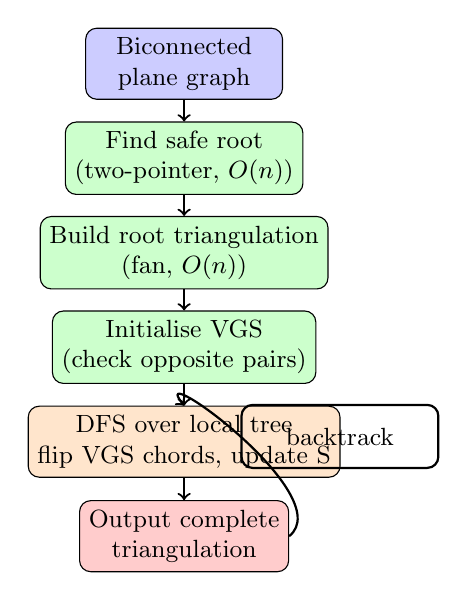
\begin{tikzpicture}[node distance=1.2cm, every node/.style={rectangle, draw, rounded corners, align=center, font=\small, minimum width=2.5cm, minimum height=0.8cm}]
        \node (input) [fill=blue!20] {Biconnected\\plane graph};
        \node (safe) [below of=input, fill=green!20] {Find safe root\\ (two-pointer, \(O(n)\))};
        \node (root) [below of=safe, fill=green!20] {Build root triangulation\\ (fan, \(O(n)\))};
        \node (vgs) [below of=root, fill=green!20] {Initialise VGS\\ (check opposite pairs)};
        \node (dfs) [below of=vgs, fill=orange!20] {DFS over local tree\\ flip VGS chords, update S};
        \node (output) [below of=dfs, fill=red!20] {Output complete\\ triangulation};
        \draw[->, thick] (input) -- (safe);
        \draw[->, thick] (safe) -- (root);
        \draw[->, thick] (root) -- (vgs);
        \draw[->, thick] (vgs) -- (dfs);
        \draw[->, thick] (dfs) -- (output);
        \draw[->, thick, bend right] (output) to[out=270,in=0] node[right] {backtrack} (dfs);
    \end{tikzpicture}
    \caption{High-level flow of the algorithm. Each face is processed in a recursive DFS; the global chord set \(S\) is updated along the path.}
    \label{fig:algorithm_flow}
\end{figure}

\section{Theoretical Significance}
\label{sec:significance}

This work makes several theoretical contributions to the field of combinatorial enumeration of plane graph triangulations:

\begin{itemize}
    \item It shows that constant-time enumeration is achievable for the strictly larger class of biconnected plane graphs, not just for triconnected graphs.
    \item The safe root concept provides a general method for initialising a genealogical tree in the presence of external constraints (chords from previous faces).
    \item The persistence lemma (Lemma~\ref{lem:persistence}) and the resulting pruning strategy are applicable to other recursive decomposition problems where certain substructures are never modified.
    \item The two-pointer safe root finding algorithm is a novel application of planarity to linear-time constraint satisfaction.
\end{itemize}

\section{Limitations}
\label{sec:limitations_conclusion}

Our algorithm has two main limitations:

\begin{enumerate}
    \item \textbf{Graph class:} It only works for biconnected plane graphs. 
    For 1-connected graphs, faces may contain repeated vertices, and a safe root may not exist (Chapter~\ref{ch:one_connected}). 
    Extending to 1-connected graphs remains an open problem.
    
    \item \textbf{Labeled graphs only:} The algorithm generates all labeled triangulations (vertices are distinguished). 
    For unlabeled graphs, additional symmetry-breaking is needed to avoid isomorphic duplicates, which we have not implemented.
\end{enumerate}

\section{Concluding Remarks}
\label{sec:concluding_remarks}

We have presented an algorithm that generates all triangulations of a biconnected plane graph in optimal amortised time and linear space. 
The algorithm combines the genealogical tree approach for cycles with a novel face-by-face processing strategy, safe root selection, and dynamic global chord management. 
Experimental results confirm the theoretical predictions and demonstrate practical efficiency.

We believe that the ideas introduced in this thesis—safe root vertices, persistent chord pruning, and the valid generating set—will find applications in other enumeration problems for planar graphs and beyond. 
Future work includes extending the algorithm to 1-connected graphs via biconnected decomposition, adapting it to 1-planar graphs, and developing a parallel version. 
We hope that this work contributes to a deeper understanding of triangulation enumeration and inspires further research in combinatorial generation for planar structures.